
\chapter{Peripheral Swedish: geographic, historical and linguistic background}
\section{ Geography}

Sweden is traditionally divided into three major regions: Götaland, Svealand, and Norrland (see \figref{map:1}), and since these regions are mentioned in all weather forecasts, people are quite aware of the division. Götaland and Svealand are commonly presumed to correspond to the lands of the two ethnic groupings Götar and Svear which are believed to form the basis of the Swedish people.  However, present-day Götaland also includes the originally Danish and Norwegian provinces that became Swedish territory in the 17\textsuperscript{th} century. The third region, Norrland – literally “the north land” – has no connection with any specific ethnic grouping (although it houses Finnish and Saami minorities), but rather represents the peripheral areas to the north that were colonized by Swedish-speaking people rather late. Although its area (242,735 sq. kms) is more than half of that of Sweden, it has only about 13 per cent of the population (1.15 million in 2003) and a population density of about 5 persons per square kilometre (compared to about 30 for the rest of Sweden). Sweden’s record as a traditional colonial power is somewhat meagre, but Norrland has undoubtedly served the role of a substitute for overseas colonies, much like Siberia for the Russian empire. Today, in spite of its impressive natural resources (such as forests, iron ore and water power), Norrland is plagued by high rates of unemployment and decreasing population figures. 

The delineation of Norrland, as officially defined, is somewhat arbitrary, however. Historically, the southernmost province of Norrland, Gästrikland, was part of Svealand. But what is more important is that a large number of natural and cultural borderlines all bisect Sweden in roughly the same way, with the northern part including not only Norrland but also a large part of Svealand, notably the province of Dalarna, and parts of the provinces of Värmland and Västmanland. This cluster of borderlines is usually referred to by the Latin phrase \textstyleLinguisticExample{limes norrlandicu}\textstyleLinguisticExample{s} ‘the Norrlandic border’ (see \figref{map:1}), and coincides fairly well with the isotherm for a January average temperature of \nobreakdash-7°C. From the point of view of vegetation, \textstyleLinguisticExample{limes norrlandicus} delimits the “northern coniferous area”, which is part of the huge taiga belt covering most of northern Eurasia. Deciduous trees such as oak and ash stop at the \textstyleLinguisticExample{limes norrlandicus}, and so did towns and nobility in the Middle Ages. The \textstyleLinguisticExample{limes norrlandicus} also coincides with the southern limit of the North Scandinavian transhumance system (seasonal movement of cattle, Swedish \textit{fäbodväsendet}), further indicating the impact of this natural borderline on cultural practices.\footnote{ The Swedish term \textstyleLinguisticExample{fäbod }is translated in dictionaries as “summer pasture”, but this is a bit misleading since it refers to the whole complex of buildings and surrounding grazing fields that were used during the summer period. For this reason, I use the term “shieling”\textstyleLinguisticExample{, }which has an analogous use in parts of Britain, as a translation of \textstyleLinguisticExample{fäbod} and the corresponding vernacular terms (such as Elfdalian \textstyleLinguisticExample{buðer}).} This border is still very much a socio-cultural reality today, as evidenced by the fact that municipalities with less than 40 per cent in favour of Sweden joining the European Union in the 1994 referendum were overwhelmingly situated north of the \textit{limes norrlandicus}.

For simplicity, I shall refer to the area north of the \textstyleLinguisticExample{limes norrlandicus} as “Northern Sweden”. This term, then, is not synonymous to “Norrland”. \textstyleLinguisticExample{Limes norrlandicus} is not frequently mentioned in the Swedish dialectological literature, but some isoglosses do follow it quite closely. Compare e.g. \textstyleLinguisticExample{limes norrlandicus} as shown in \figref{map:1} with the southern limit of the “North Scandinavian medial affrication” as shown in \figref{map:22} (page 203) and the southern limit of the area with predominantly postposed pronominal possessors in \figref{map:21} (page 199). It is clear that the natural conditions of Northern Sweden have not only influenced the inhabitants’ way of living but have also – indirectly – been important for linguistic developments.

The linguistic phenomena discussed in this book occur mainly in Northern Sweden, as defined in the preceding paragraph, as well as in the Trans-Baltic parts of the Scandinavian dialect continuum (Finland, Estonia), particularly the Finnish province of Österbotten (Ostrobothnia, Pohjanmaa), and extending in some cases also to the islands of Gotland and Öland in the southern Baltic. I shall refer to this area as the \textbf{Peripheral Swedish }area. It has been pointed out to me that the term “peripheral” may be interpreted as having negative associations; this is most certainly not the intention here – in particular I do not want to imply that the vernaculars spoken in the Peripheral Swedish area have a peripheral role to play relative to standard or acrolectal varieties.\footnote{ The EU-supported Northern Periphery programme () happens to delimit its area of activity in a way that makes it coincide quite closely in Sweden with the Peripheral Swedish area as I have defined it. (See map at http://www.northernperiphery.eu.} 

\section{ Administrative, historical and dialectological divisions}

The first-level administrative units in Sweden and Finland are called \textstyleLinguisticExample{län} (Swedish) or \textstyleLinguisticExample{lääni} (Finnish). These will be referred to as “counties”. The second-level unit is called \textstyleLinguisticExample{kommun} in Swedish and \textstyleLinguisticExample{kunta} in Finnish, translated as “municipalities”. However, in dialectology, the traditional partitioning into \textstyleLinguisticExample{landskap} (translated as “province”), \textstyleLinguisticExample{härad} (translated as “judicial district”) and \textstyleLinguisticExample{socken} (translated as “parish”) is more useful. 

I will use the Swedish toponyms for all these units throughout. When referring to dialects or dialect areas, however, I will sometimes use Latinized forms such as “Dalecarlian” and “Westrobothnian”, particularly in those cases where the dialectological unit does not coincide with the geographical one.

Examples from individual parishes will in general be identified by the name of the parish (in some cases also by a village name), followed by an abbreviation for the dialect area or province in parentheses. Sometimes, however, sources use traditional denominations of vernaculars, which may cover areas which are larger or smaller than a parish (e.g. \textit{Lulemål}, \textit{Önamål}) – these are then cited in italics. For the vernacular spoken in Älvdalen, Dalarna, I use the Latinized name “Elfdalian”, which is currently gaining ground as an English term, although it has received a competitor in the alternative name “Övdalian”.

\begin{figure}[h]

%\begin{styleBeschriftung}
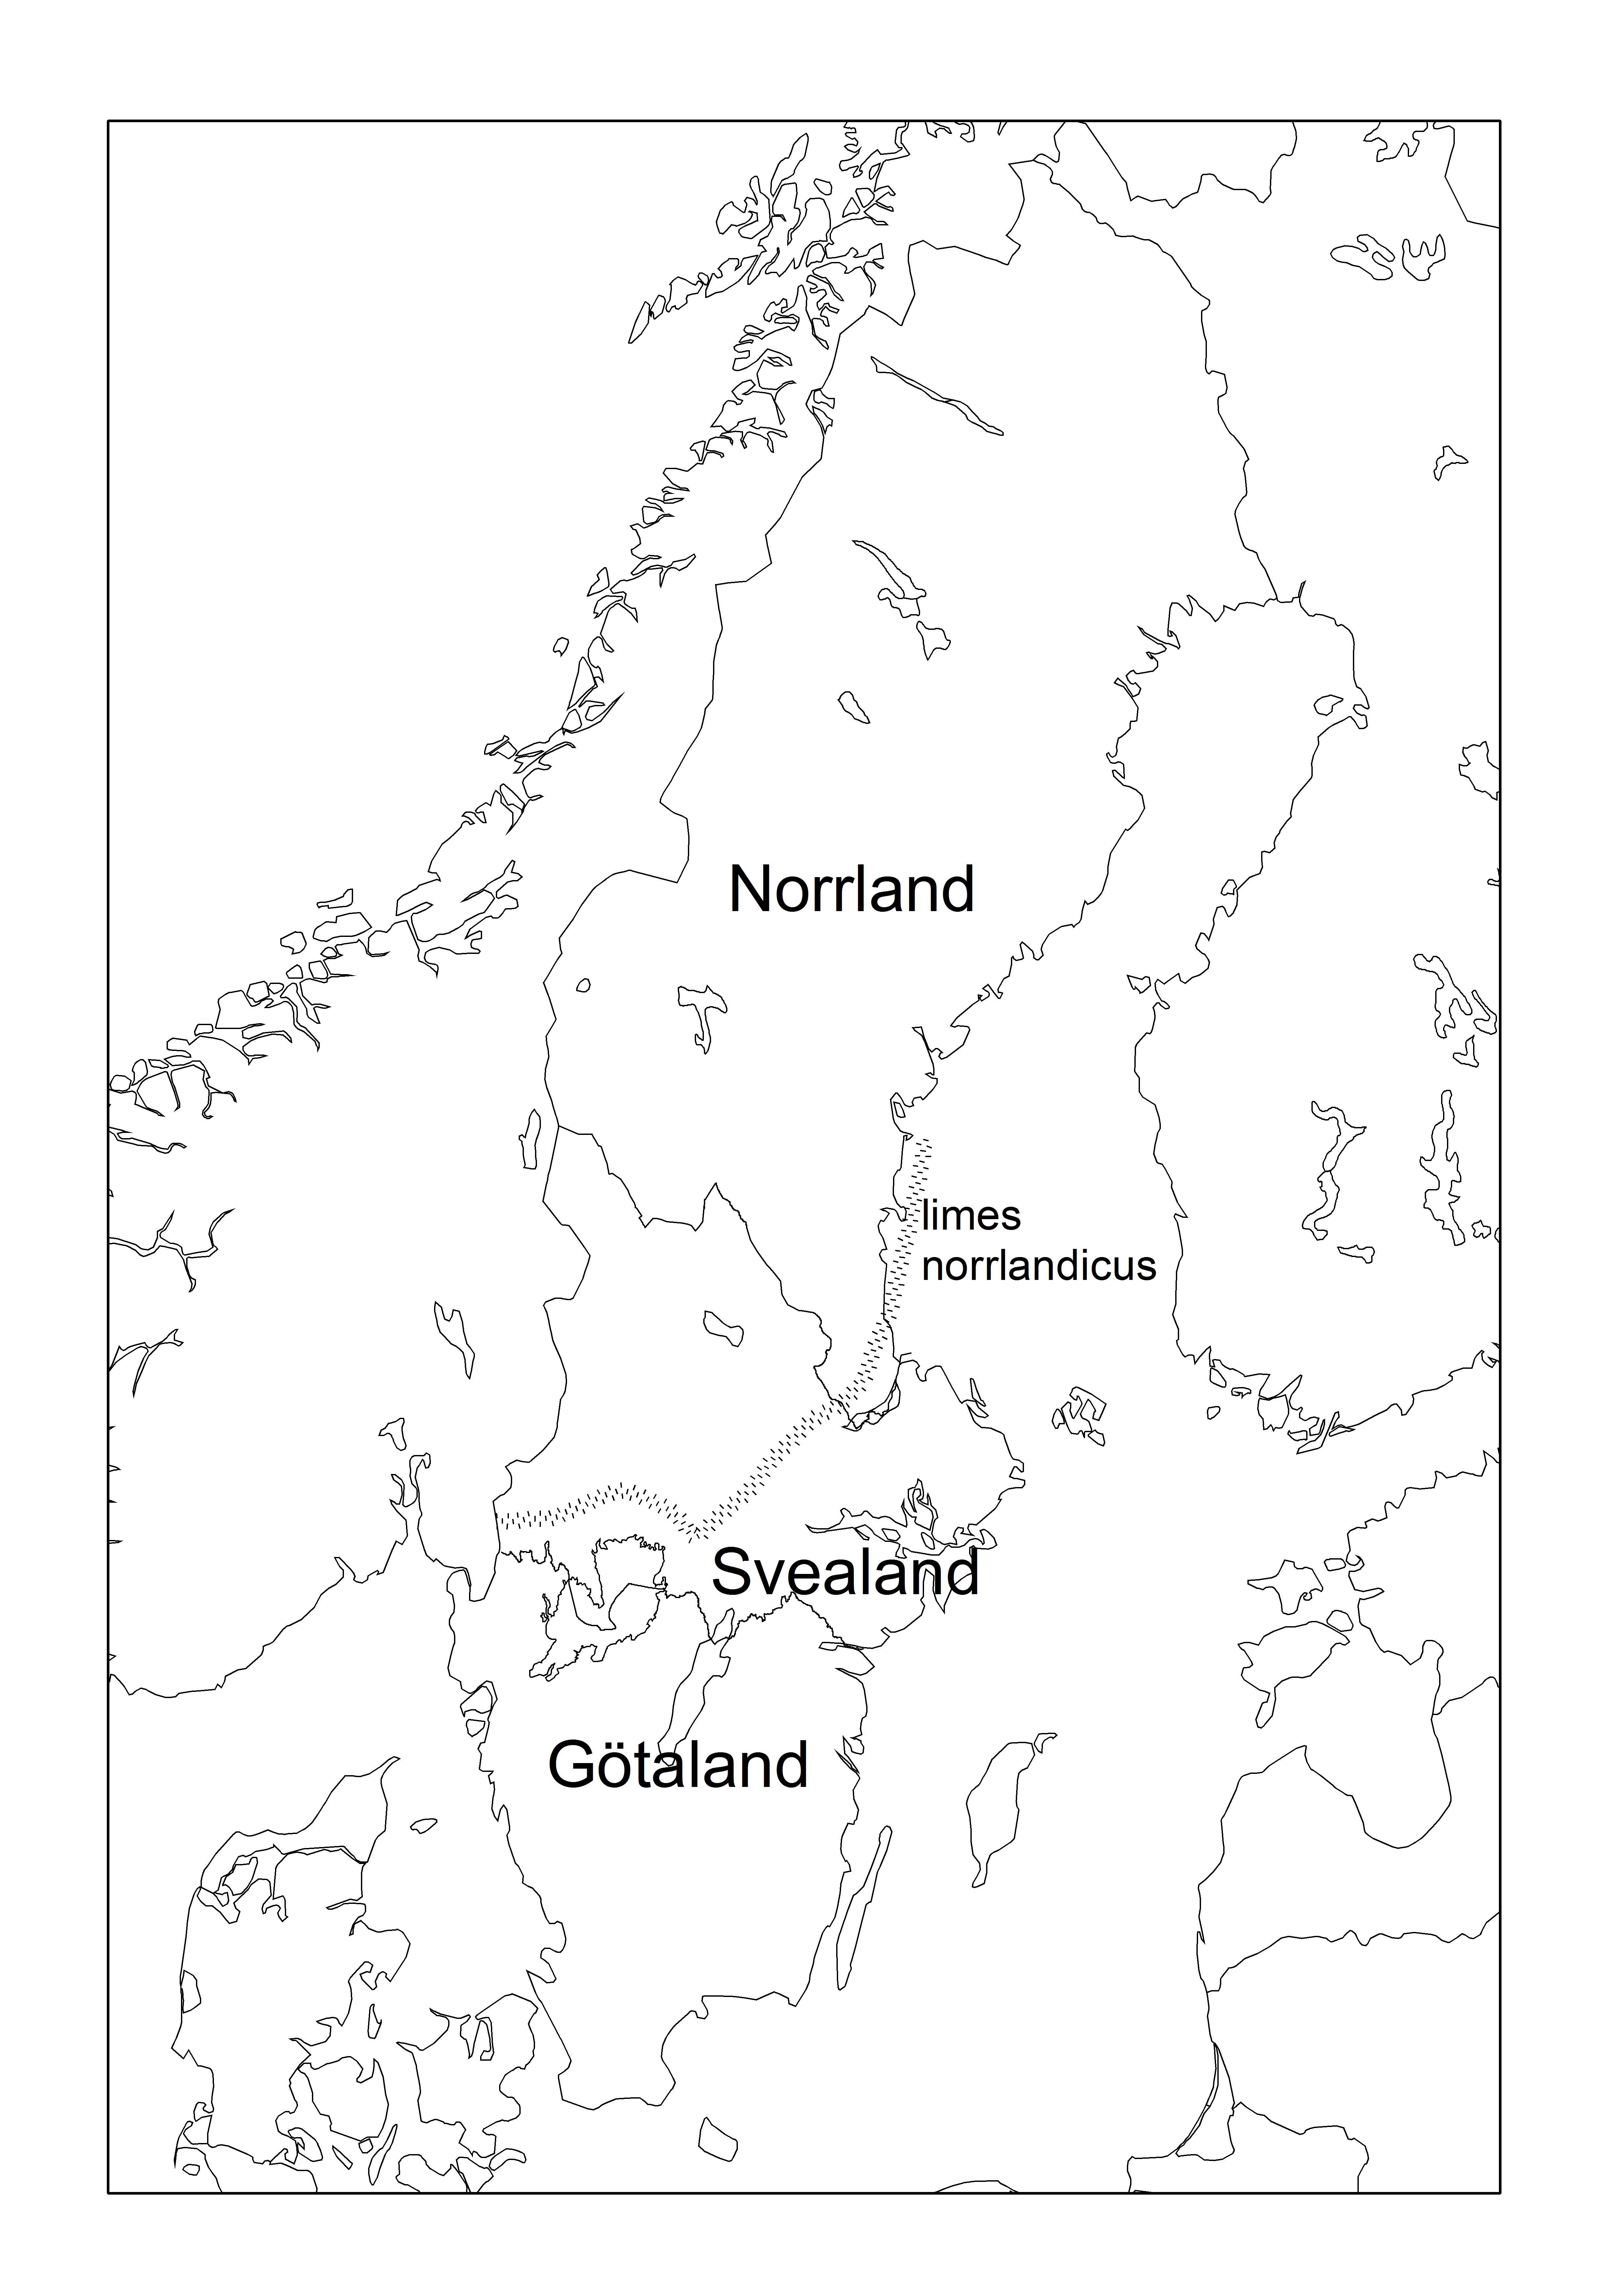
\includegraphics[height=.3\textheight]{figures/2_TraditionalGeographicdivisions}
\caption{Traditional geographical divisions in Sweden.}
\label{map:1}

\end{figure}

\begin{figure}[h]
\includegraphics[height=.3\textheight]{figures/3_SwedishDialectAreas}
\caption{Swedish dialect areas according to \citet{Wessén1966}. Larger print: major areas, smaller print: minor areas. Grey dots indicate parishes within the traditional Swedish-speaking area. (This also gives a fairly adequate idea of the population density.) Notice that “East Swedish dialects” are called “Trans-Baltic” in this text.}
\label{map:2}

\end{figure}

\begin{figure}[h]

%\begin{styleBeschriftung}
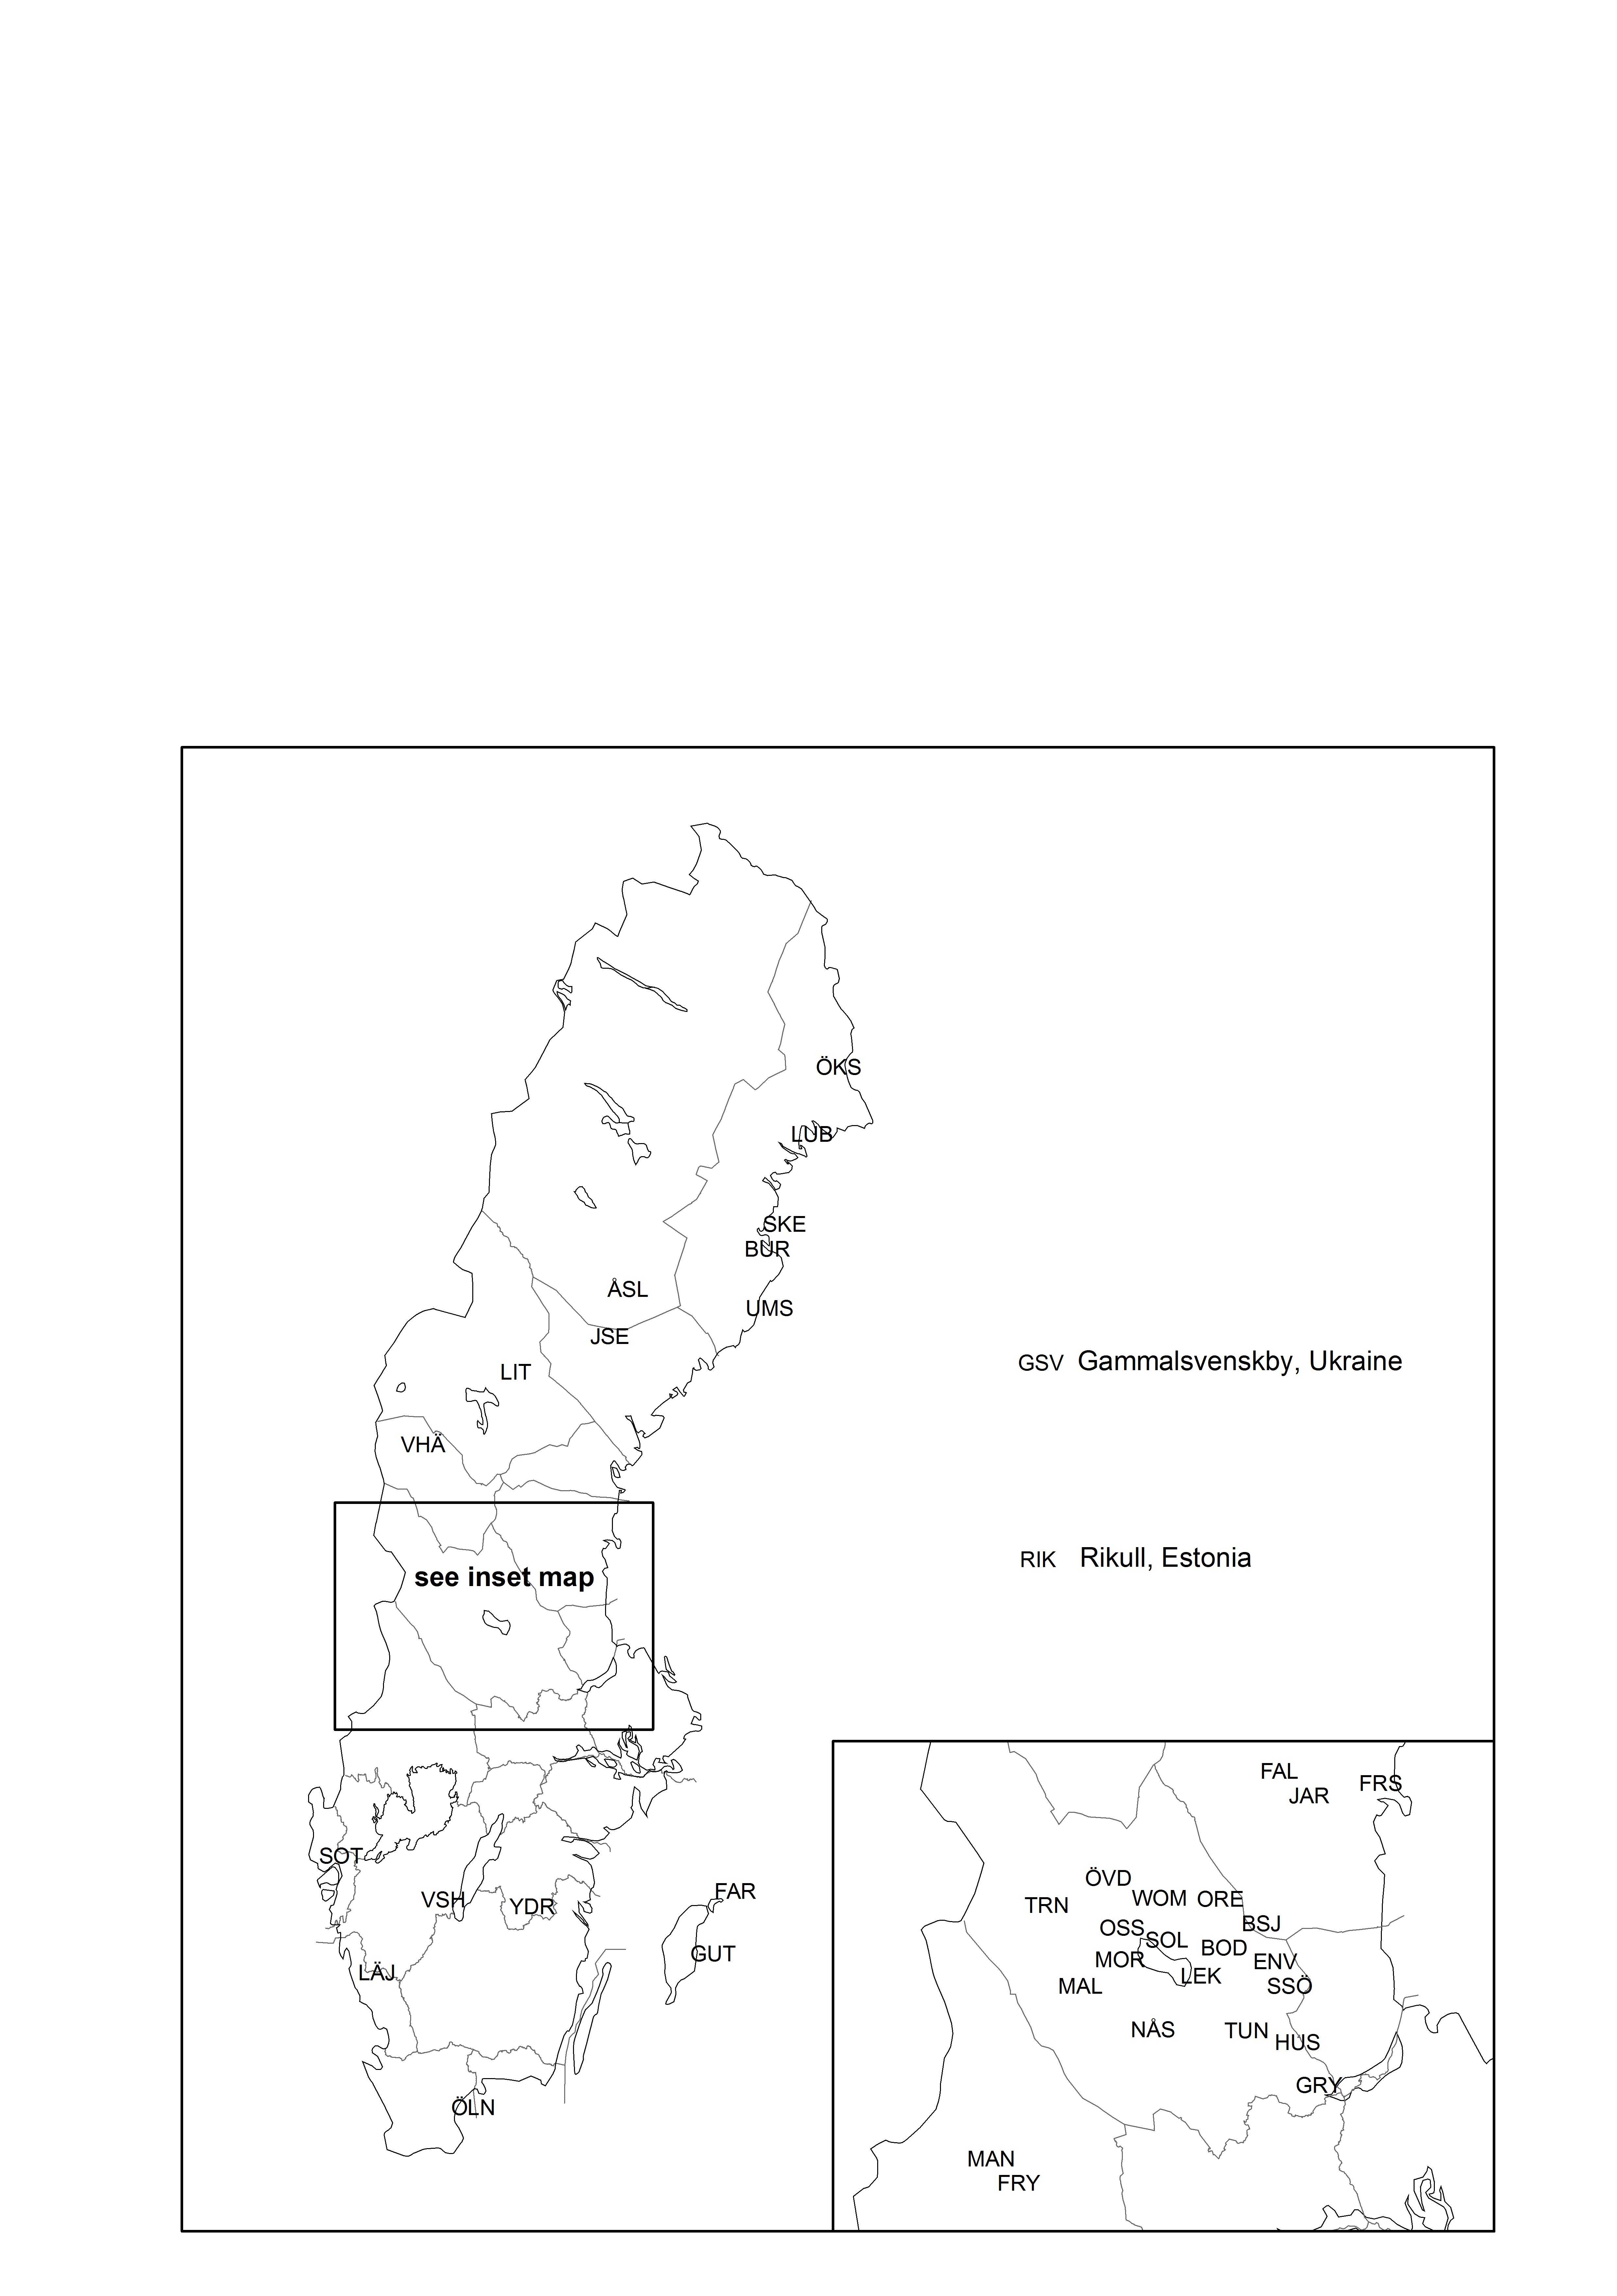
\includegraphics[height=.3\textheight]{figures/4_VernacularsrepresentedCatCorpus}
\caption{Vernaculars represented in the Cat Corpus.}
\label{map:3}

\end{figure}

\begin{figure}[h]

%\begin{styleBeschriftung}
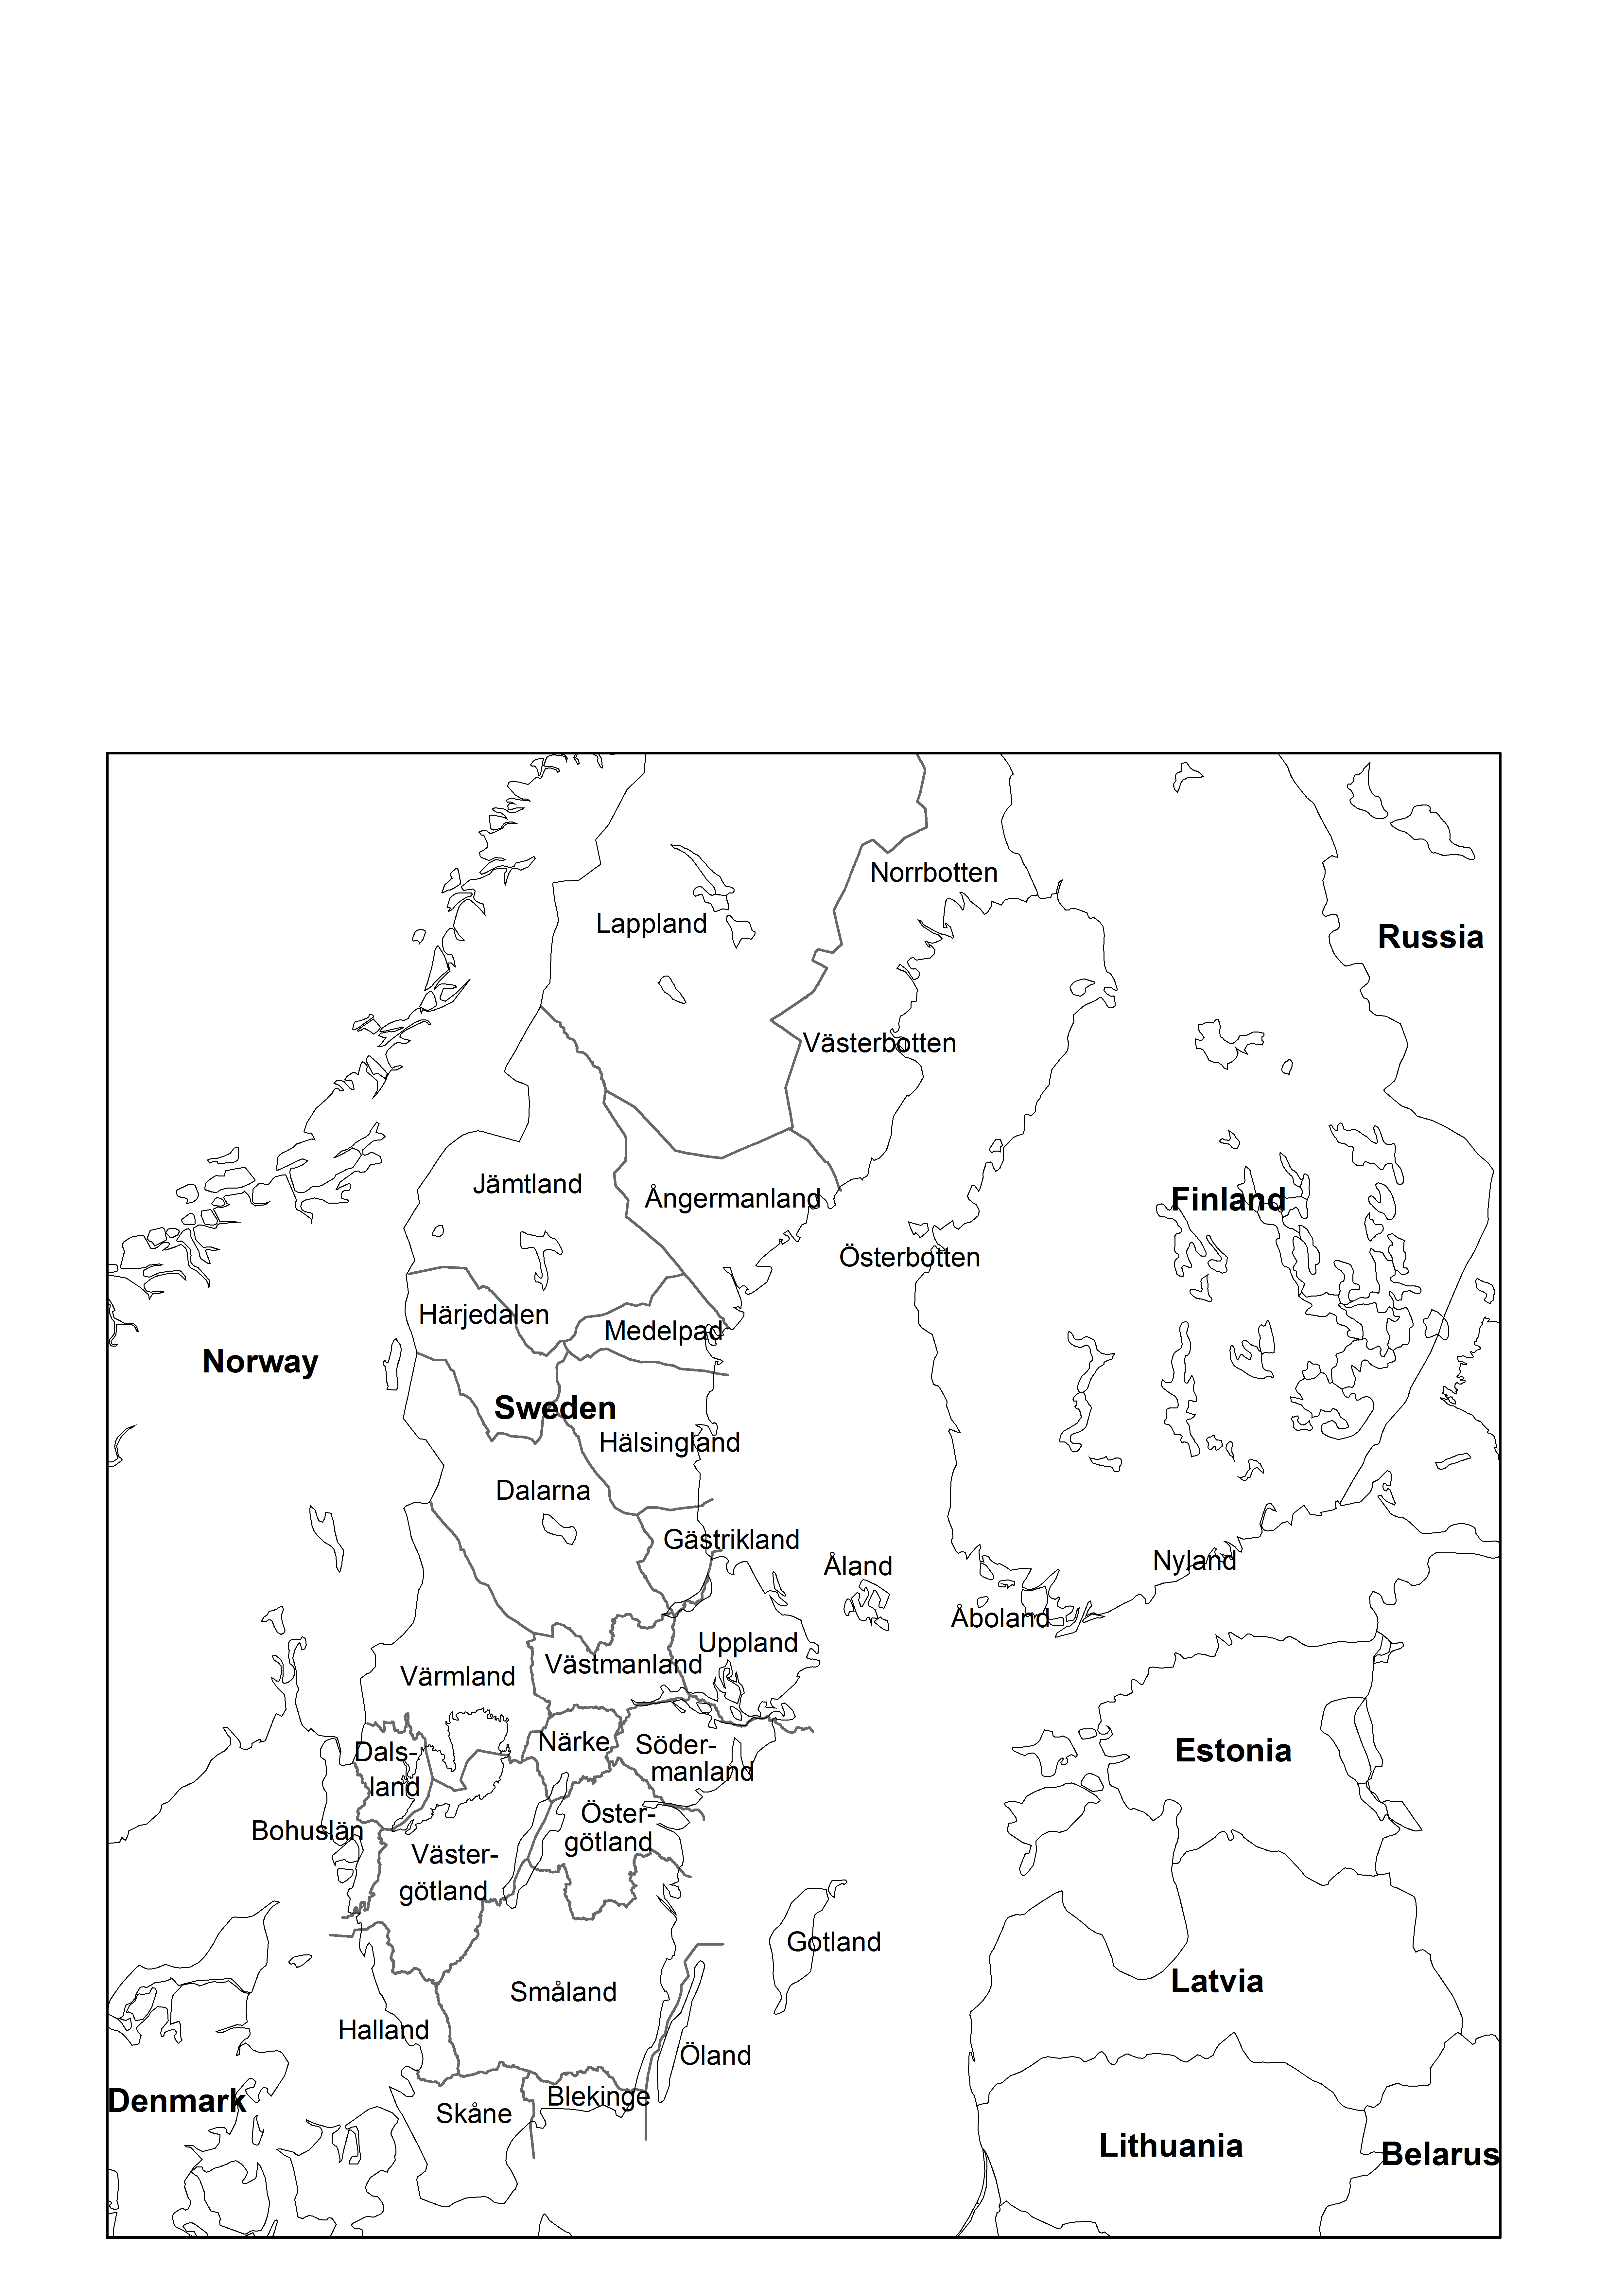
\includegraphics[height=.3\textheight]{figures/5_SwedishProvinces}
\caption{Swedish provinces (\textit{landskap}).}
\label{map:4}

\end{figure}

\begin{figure}[h]

\textbf{Abbreviations for provinces in Sweden south of}\textstyleLinguisticExample{ limes norrlandicus}

Blekinge  Bl  Södermanland  Sö

Bohuslän  Bo  Uppland  Up

Dalsland  Dl  Värmland  Vm

Gotland  Go  Västergötland  Vg

Halland  Hl  Västmanland  Vl

Närke  Nä  Öland  Öl

Skåne  Sk  Östergötland  Ög

Småland  Sm    

\end{figure}

\begin{figure}[h]

%\begin{styleBeschriftung}
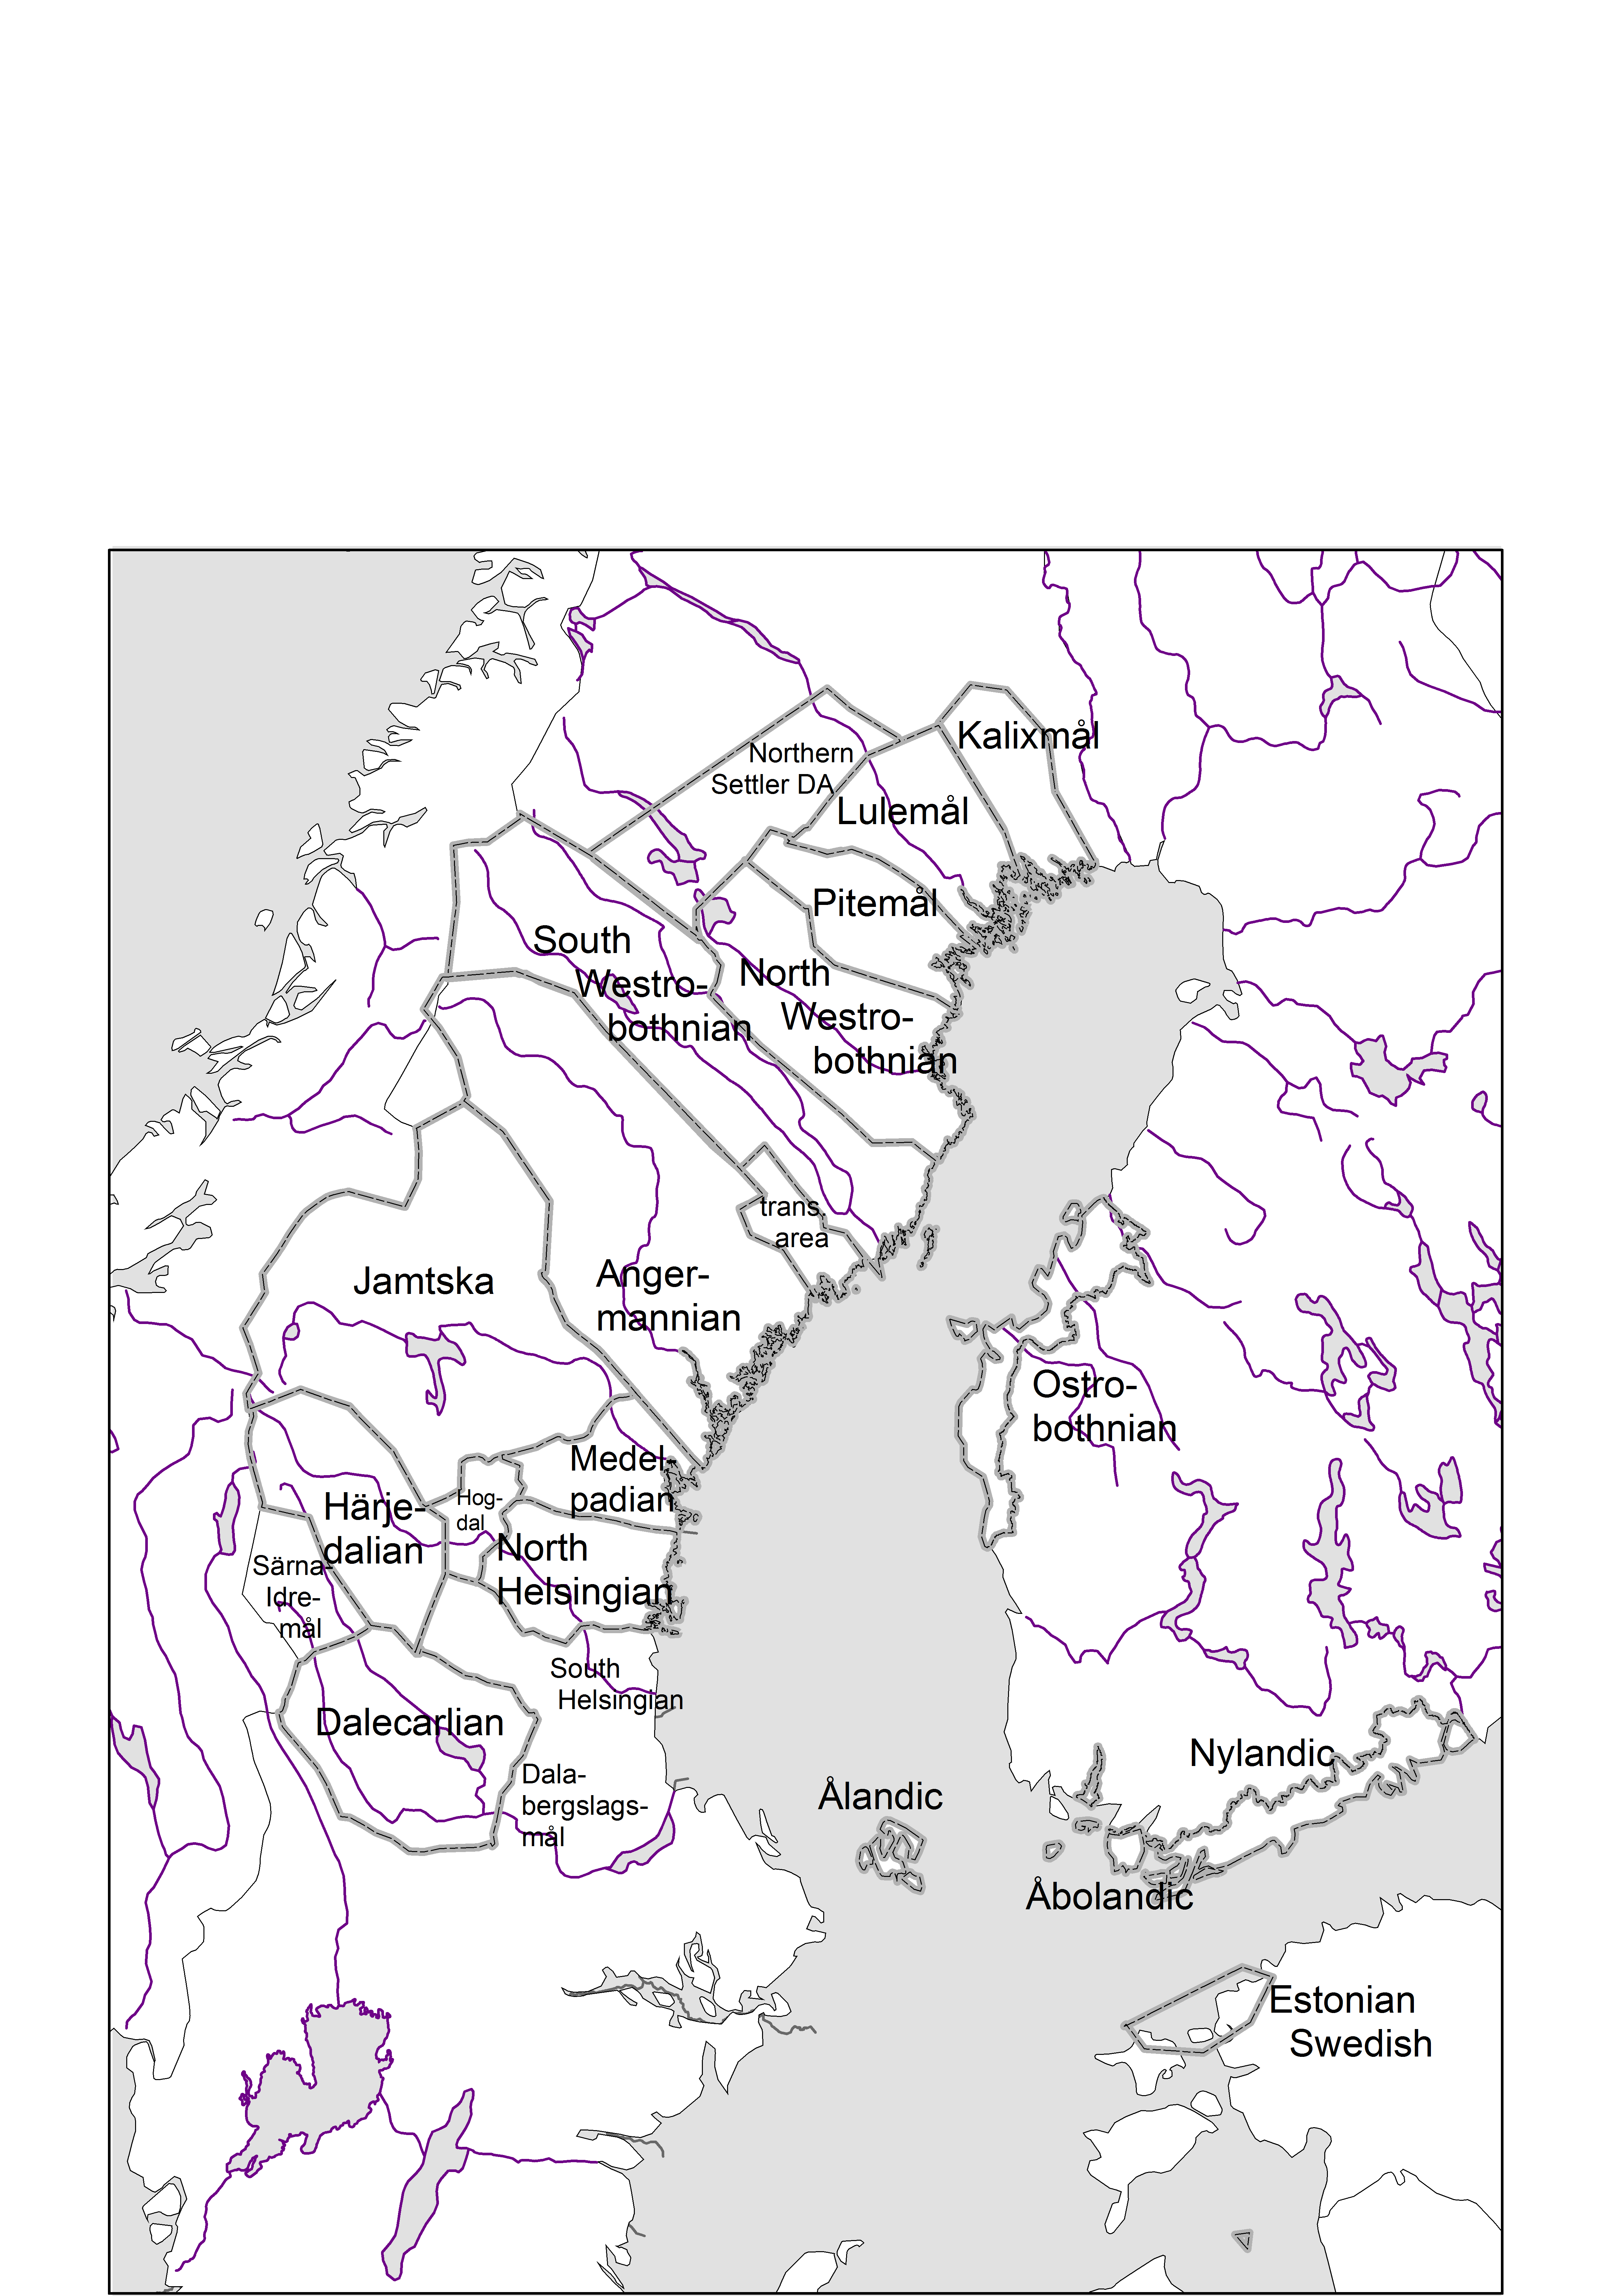
\includegraphics[height=.3\textheight]{figures/6_DialectAreas}
\caption{Dialect areas in the Peripheral Swedish Area.}
\label{map:5}

\end{figure}
 

\begin{table}
\caption{Vernacular groupings in and around the Peripheral Swedish area}
%   \setlength{\parsep}{0pt}
\small 
\begin{tabular}{p{.5\textwidth}l}
\lsptoprule
Norrbothnian (norrbottniska) &
      \parbox{.5\textwidth}{
	  \begin{itemize}
  \setlength{\itemsep}{0pt}
	  \item  \textit{Kalixmål} (Kx)
	  \item  \textit{Lulemål} (Ll)
	  \item  \textit{Pitemål} (Pm)
	  \end{itemize}
      }
\\
Westrobothnian (västerbottniska) &
      \parbox{.5\textwidth}{
	  \begin{itemize}
  \setlength{\itemsep}{0pt}
	  \item Northern Westrobothnian (nordvästerbottniska) (NVb)
	  \item Southern Westrobothnian
		(sydvästerbottniska) (SVb)
	  \item Angermannian-Westrobothnian
		transitional area (övergångsmål) (ÅV)
	  \end{itemize}
}
\\
Northern Settler dialect area (Nm)  
\\
Angermannian (ångermanländska) (Åm)  
\\
\textit{Jamtska (jämtska)} (Jm)  
\\
Medelpadian (medelpadska) (Md)  
\\
Helsingian (hälsingska) (Hä)  
\\
Dalecarlian ((egentligt) dalmål) &
      \parbox{.5\textwidth}{
	  \begin{itemize} 
  \setlength{\itemsep}{0pt}
	      \item Ovansiljan (Os)
	      \item Västerdalarna (Vd)
	      \item Nedansiljan (Ns)
	  \end{itemize}
}
\\
Dalabergslagsmål (Be)  
\\
Ostrobothnian (österbottniska) &
      \parbox{.5\textwidth}{
	  \begin{itemize} 
  \setlength{\itemsep}{0pt}
	  \item Northern Ostrobothnian (NOb)
	  \item Central Ostrobothnian (COb)
	  \item Southern Ostrobothnian (SOb)
	  \end{itemize}
}
\\
Southern Finland Swedish vernaculars &
      \parbox{.5\textwidth}{
	  \begin{itemize} 
  \setlength{\itemsep}{0pt}
	   \item  Åbolandic (Åb)
	  \item Nylandic (Ny)
	  \item Ålandic (Ål)
	  \end{itemize}
}
\\
Estonian Swedish vernaculars (including Gammalsvenskby, Ukraine) (Es)  
\\
“Norwegian” vernaculars  &
      \parbox{.5\textwidth}{
	  \begin{itemize} 
  \setlength{\itemsep}{0pt}
\item  Härjedalian (Hd)
\item \textit{Särna-Idremål} (SI)\\
	  \end{itemize}
}\\
\lspbottomrule
\end{tabular}
\end{table}


\section{ Linguistic situation}
\subsection{ Scandinavian in general}

According to the traditional view, the Scandinavian languages (also referred to as “Nordic” and “North Germanic”) are divided into two branches, West Scandinavian, comprising Icelandic, Faroese, and Norwegian, and East Scandinavian, comprising Danish and Swedish. The two branches are thought to have formed around 1000 AD. This classification is not very easy to apply to the present-day languages, however. Due to the prevalence of Danish in Norway during the half millennium of Danish rule there, and the efforts during the 19\textsuperscript{th} century to re-create Norwegian as a written language, Norwegian today has two written standards, \textstyleLinguisticExample{bokmål} and \textstyleLinguisticExample{nynorsk,} with the former being fairly close to Danish and the latter being based mainly on rural vernaculars. Consequently, in some treatments \textstyleLinguisticExample{bokmål} is seen as an East Scandinavian language and \textstyleLinguisticExample{nynorsk} as a West Scandinavian language, which is counterintuitive since both varieties are not only very close to each other but also much more similar to Danish and Swedish than to Modern Icelandic. If one also takes the various spoken vernaculars in continental Scandinavia into account, it becomes clear that the standard languages Danish, Swedish, and Norwegian Bokmål and vernaculars spoken in the insular part of Denmark, urbanized areas in Norway, and Sweden south of the \textstyleLinguisticExample{limes norrlandicus}, form a cluster of relatively closely connected (and more or less mutually intelligible) varieties, to be referred to in the following as \textbf{Central Scandinavian}\textbf{.}. The reason for the closeness of the Central Scandinavian varieties is then not so much common origin as intensive language contact over prolonged periods. On the other hand, the spoken varieties in the rest of Continental Scandinavia, that is, Jutland in Denmark, most of rural Norway and the Peripheral Swedish Area, together with “Insular North Germanic”, i.e. Icelandic and Faroese, stand apart from Central Scandinavian; and, although there is great diversity among them, they tend to share many “conservative” traits inherited from Old Nordic which are no longer found in Central Scandinavian. In addition, there are also innovations that cover large parts of the peripheral areas which will be of particular interest to what follows. 

\subsection{ Swedish}
\label{sec:2.3.2}

The area where varieties traditionally regarded as “Swedish dialects” are spoken includes all of Sweden (except the Saami-speaking and Finnish-speaking areas in the very north), the Åland islands (Finnish \textstyleLinguisticExample{Ahvenanmaa}), two separate areas along the Finnish coast, and a small area on the coast of Estonia. I shall refer to this as the \textbf{Swedish dialect area.} It is shown in \figref{map:2}together with the standard division into six dialect groupings following \citet[II:170]{Wessén1966}: 

%\begin{listLFOviileveli}
\begin{itemize}
\item 

%\begin{styleListeii}
Southern dialects (\textit{sydsvenska mål})

%\end{styleListeii}

\item 

%\begin{styleListeii}
Göta dialects (\textit{götamål})

%\end{styleListeii}

\item 

%\begin{styleListeii}
Svea dialects (\textit{sveamål})

%\end{styleListeii}

\item 

%\begin{styleListeii}
Norrlandic dialects (\textit{norrländska mål})

%\end{styleListeii}

\item 

%\begin{styleListeii}
East Swedish dialects (\textit{östsvenska mål})

%\end{styleListeii}

\item 

%\begin{styleListeii}
Gotlandic dialects (\textit{gotländska mål})

%\end{styleListeii}

%\end{listLFOviileveli}
\end{itemize}

Notice that “East Swedish” does not refer to dialects spoken in the eastern parts of Sweden but rather to those spoken east of the Baltic. For this reason the less confusing term “Trans-Baltic” was introduced in \citet{Rendahl2001} and will be used here.

Wessén identifies a transitional belt between the Svea and Göta dialects in the area comprised of the western part of Södermanland, Närke, all of Östergötland except the south-western part, northeast Småland, and Öland (see \figref{map:4} for the provinces). For this reason, he says, the Svea dialects should be divided into two sub-areas: (i) the dialects in the transitional belt, referred to as “Central Swedish dialects” (\textstyleLinguisticExample{mellansvenska mål}), (ii) the rest, i.e. Uppland, Gästrikland, southern Hälsingland, south-eastern Dalarna, eastern Västmanland, and northern and eastern Södermanland, making up the “Upper Swedish” dialects (\textstyleLinguisticExample{uppsvenska mål}). He adds that the dialects of Upper Dalarna (\textit{egentligt dalmål} ‘Dalecarlian proper’) \label{bkm:wessenquote}“have a special position”,\footnote{\textsuperscript{ }“En särställning intar det egentliga dalmålet i Öster- och Västerdalarne, med sin mycket ålderdomliga prägel och sin starka splittring i underarter” (p. 30).  (Wessén’s map says simply \textit{dalmål} ‘Dalecarlian’.)} but does not specify if they should be counted as Upper Swedish or not.

The northern part of the Swedish-speaking area has been most controversial with respect to how it should be divided into dialect areas. Before the advent of modern dialectology in the 19\textsuperscript{th} century, the traditional opinion seems to have been that there were two major Swedish dialects, “Svea” and “Göta”. The former would then also include the vernaculars of Dalarna and Norrland (and presumably also the Trans-Baltic varieties). Another way of slicing the cake was proposed by the Swedish dialectologist Johan Lundell (1880, 1901) who united most Norwegian dialects together with those spoken in Norrland, Dalarna, Västmanland, Finland and Estonia into one area called “North Scandinavian”, and lumped Svea and Göta dialects together with a “Central Swedish” group (thus a wider use of this term than Wessén’s). \citet{Hesselman1905}, citing the older authors, stresses the links between the Upper Swedish dialects and those found in Northern Sweden and east of the Baltic. 

\subsection{ Norrlandic}

It is hardly surprising that there is great variation among the vernaculars of Norrland in view of the size of the region. The different parts of Norrland also have rather different histories. Norrland was first populated more or less directly after the disappearance of the continental ice sheet, but agriculture arrived relatively late. The population were mainly hunters and fishers until permanent agricultural settlements were established, which took place in the early Iron Age in middle Norrland, but only in the 13\textsuperscript{th} and 14\textsuperscript{th} centuries in the northern provinces Västerbotten and Norrbotten. Saami-speaking and Finnish-speaking populations were found more widely in this period than today. The political status of large parts of Norrland was unclear in medieval times. For example, the border between Sweden and Russia became fixed only in \textstylehitlist{1323.} The provinces of Jämtland and Härjedalen were officially part of Norway, although Jämtland’s status was rather ambiguous: ecclesiastically, it belonged to the diocese of Uppsala, and in actual practice the province may have functioned more or less as an autonomous republic. This situation is reflected linguistically in that the vernaculars of Jämtland are in various ways transitional between Swedish and Norwegian, whereas Härjedalen, which was populated from Norway at a relatively late point in time, is usually seen as being Norwegian from the dialectological point of view.

If we look at the coastal Norrlandic provinces (see \figref{map:4}), starting in the south, the vernaculars of Gästrikland, which historically did not belong to Norrland, do not differ much from those of northern Uppland. In fact, the same can be said to some extent about Hälsingland, where there appears to have been significant levelling of the vernaculars already in pre-modern times. Many phenomena that are characteristic of Northern Swedish vernaculars are found only in northern Hälsingland – for this reason \citet[230]{ÅgrenEtAl1954} regard the southern part of the province as belonging to the “Upper Swedish” area and treat northern Hälsingland as a separate dialect area. Going further north, the vernaculars grow gradually more different from Standard Swedish. The most conservative ones are probably those found in northern Västerbotten, although the varieties in Norrbotten (notably the northernmost Swedish vernacular, Överkalixmål) are more distinctive, having undergone a number of specific innovations. The Swedish dialects of the landlocked province of Lappland – the so-called “settler dialects” (\textit{nybyggarmål}) – are usually said to be closer to the standard language than the coastal vernaculars, since Swedish settlements there were generally quite late and were at least partly populated from the south. As we shall see later, however, some traits characteristic of the coastal vernaculars have also spread to the “settler dialects”. 

The dialectological map of Norrland is largely influenced by its physical geography: Norrland is crossed from west to east by a large set of rivers and since movement of people and goods has always tended to go along the rivers, there is a strong tendency for each river valley to make up a separate dialect area (see \figref{map:5}).\footnote{ \textstyleFunotentextZchn{Interestingly, the same goes also for the Saami varieties in Upper Norrland; this means that for several of the Swedish dialect areas, there is a Saami language with the same prefix to its name (Lulemål corresponds to Lule Saami etc.), although the Saami varieties are (or were) spoken in the upper parts of the river valleys and the Swedish varieties closer to the coast.}} Some dialect areas are named after the provinces, but there is considerable mismatch between the borders of the provinces and those of the dialect areas.\footnote{ I have tried to follow the map of the Norrlandic dialect areas in \citet[230]{ÅgrenEtAl1954} (reproduced also in \citet{Dahlstedt1971}). However, the transitional Angermannian-Westrobothnian area is not quite clearly delineated in this map; the border cuts straight through the parishes of Fredrika and Örträsk. It is clear from the text in the book that Örträsk should belong to the area, while Fredrika, as belonging to “Åsele lappmark”, should be counted as an Angermannian vernacular, although according to \citet[289]{ÅgrenEtAl1954}, what is spoken there is “almost standard language” (“nästan riksspråk”). } 

\subsection{ Dalecarlian}

As noted in the quotation from \citet{Wessén1966} on page 27 above, the vernaculars spoken in Upper Dalarna (Övre Dalarna), the northern part of the province of Dalarna (latinized name: Dalecarlia), have a “special position” in differing more radically from the standard languages than perhaps any Scandinavian variety and in also being extremely diverse internally. In Swedish dialectology, these vernaculars are usually referred to as \textstyleLinguisticExample{dalmål} or \textstyleLinguisticExample{egentligt dalmål }‘Dalecarlian proper’. Confusion arises from the fact that the word \textstyleLinguisticExample{dalmål} is for most Swedes associated with the characteristic accent of speakers from the southern part of the province, which belongs to the Central Swedish mining district referred to as Bergslagen. The traditional vernaculars of this part of Dalarna are referred to in the dialectological literature as \textstyleLinguisticExample{Dala-Bergslagsmål}. The term “Dalecarlian” will be used in this work to refer to “Dalecarlian proper”, that is, the traditional vernaculars of the 21 parishes of Upper Dalarna. It should be borne in mind, however, that even though Dalecarlian as a whole was during a period  assigned the status of a language in Ethnologue (\href{http://www.ethnologue.com}{{www.ethnologue.com}}), the characterization given by the foremost expert on Dalecarlian, \citet[257]{Levander1928}, is more apt: “Dalecarlian is not one language…but rather a whole world of languages”\footnote{\textsuperscript{ }“Det bör ihågkommas, att dalmålet – trots den enhet, som kan anas bakom den nuvarande mångfalden – icke är ett språk utan en hel språkvärld.”} – the parish varieties are often not mutually understandable, and the differences between villages in one and the same parish can be quite significant. 

Commonly, the Dalecarlian area is divided into three parts – Ovansiljan, Västerdalarna and Nedansiljan (see \figref{map:6}), but the actual picture is somewhat more complex. \figref{map:7} is based on a lexical comparison between vernaculars in Dalarna described in more detail in \citet{Dahl2005}. It shows that the varieties that differ most from the others (and from Standard Swedish) are found in Ovansiljan (except Ore) and northern Västerdalarna (Transtrand and Lima), these forming two fairly well delineated areas. Within Ovansiljan, the vernaculars in Älvdalen and Våmhus form a highly distinctive subarea, and Orsa also stands out as having many specific traits. Within Nedansiljan, Boda and Rättvik make up an area of their own, although it differs less dramatically from the neighbours to the south. The rest of Dalarna, including the remaining parts of Västerdalarna and Nedansiljan, is most properly regarded as a dialect continuum without clear borders. The parishes of Särna and Idre in the northern tip of the province, however, belonged to Norway until 1645 and the vernaculars there are very different from Dalecarlian, being quite similar to the Norwegian vernaculars on the other side of the border. 

\begin{figure}[h]

%\begin{styleBeschriftung}
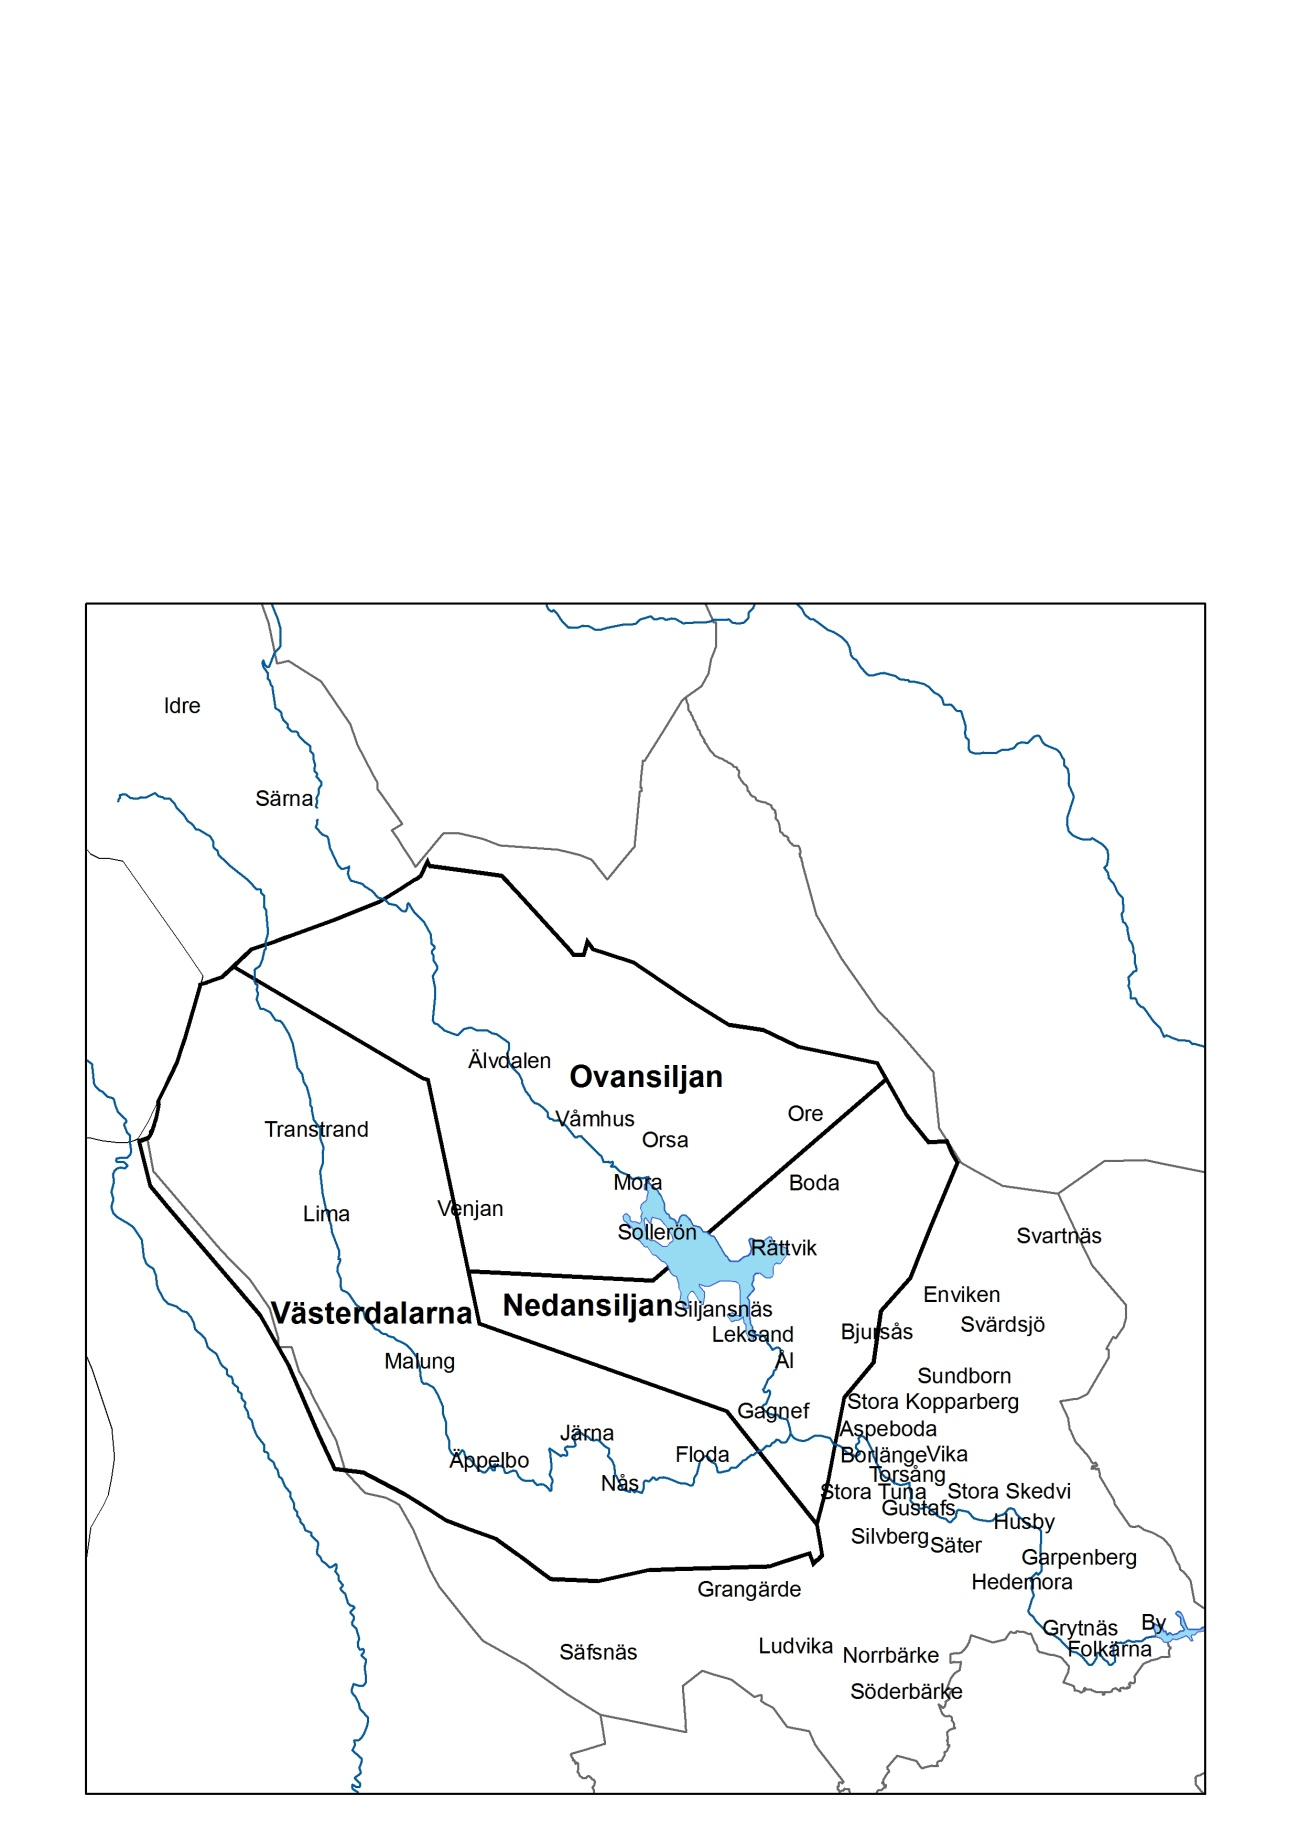
\includegraphics[height=.3\textheight]{figures/7_DialectAreasDalarnaTrad}
\caption{Dialect areas in Dalarna according to the traditional view.}
\label{map:6}

\end{figure}

\begin{figure}[h]

%\begin{styleBeschriftung}
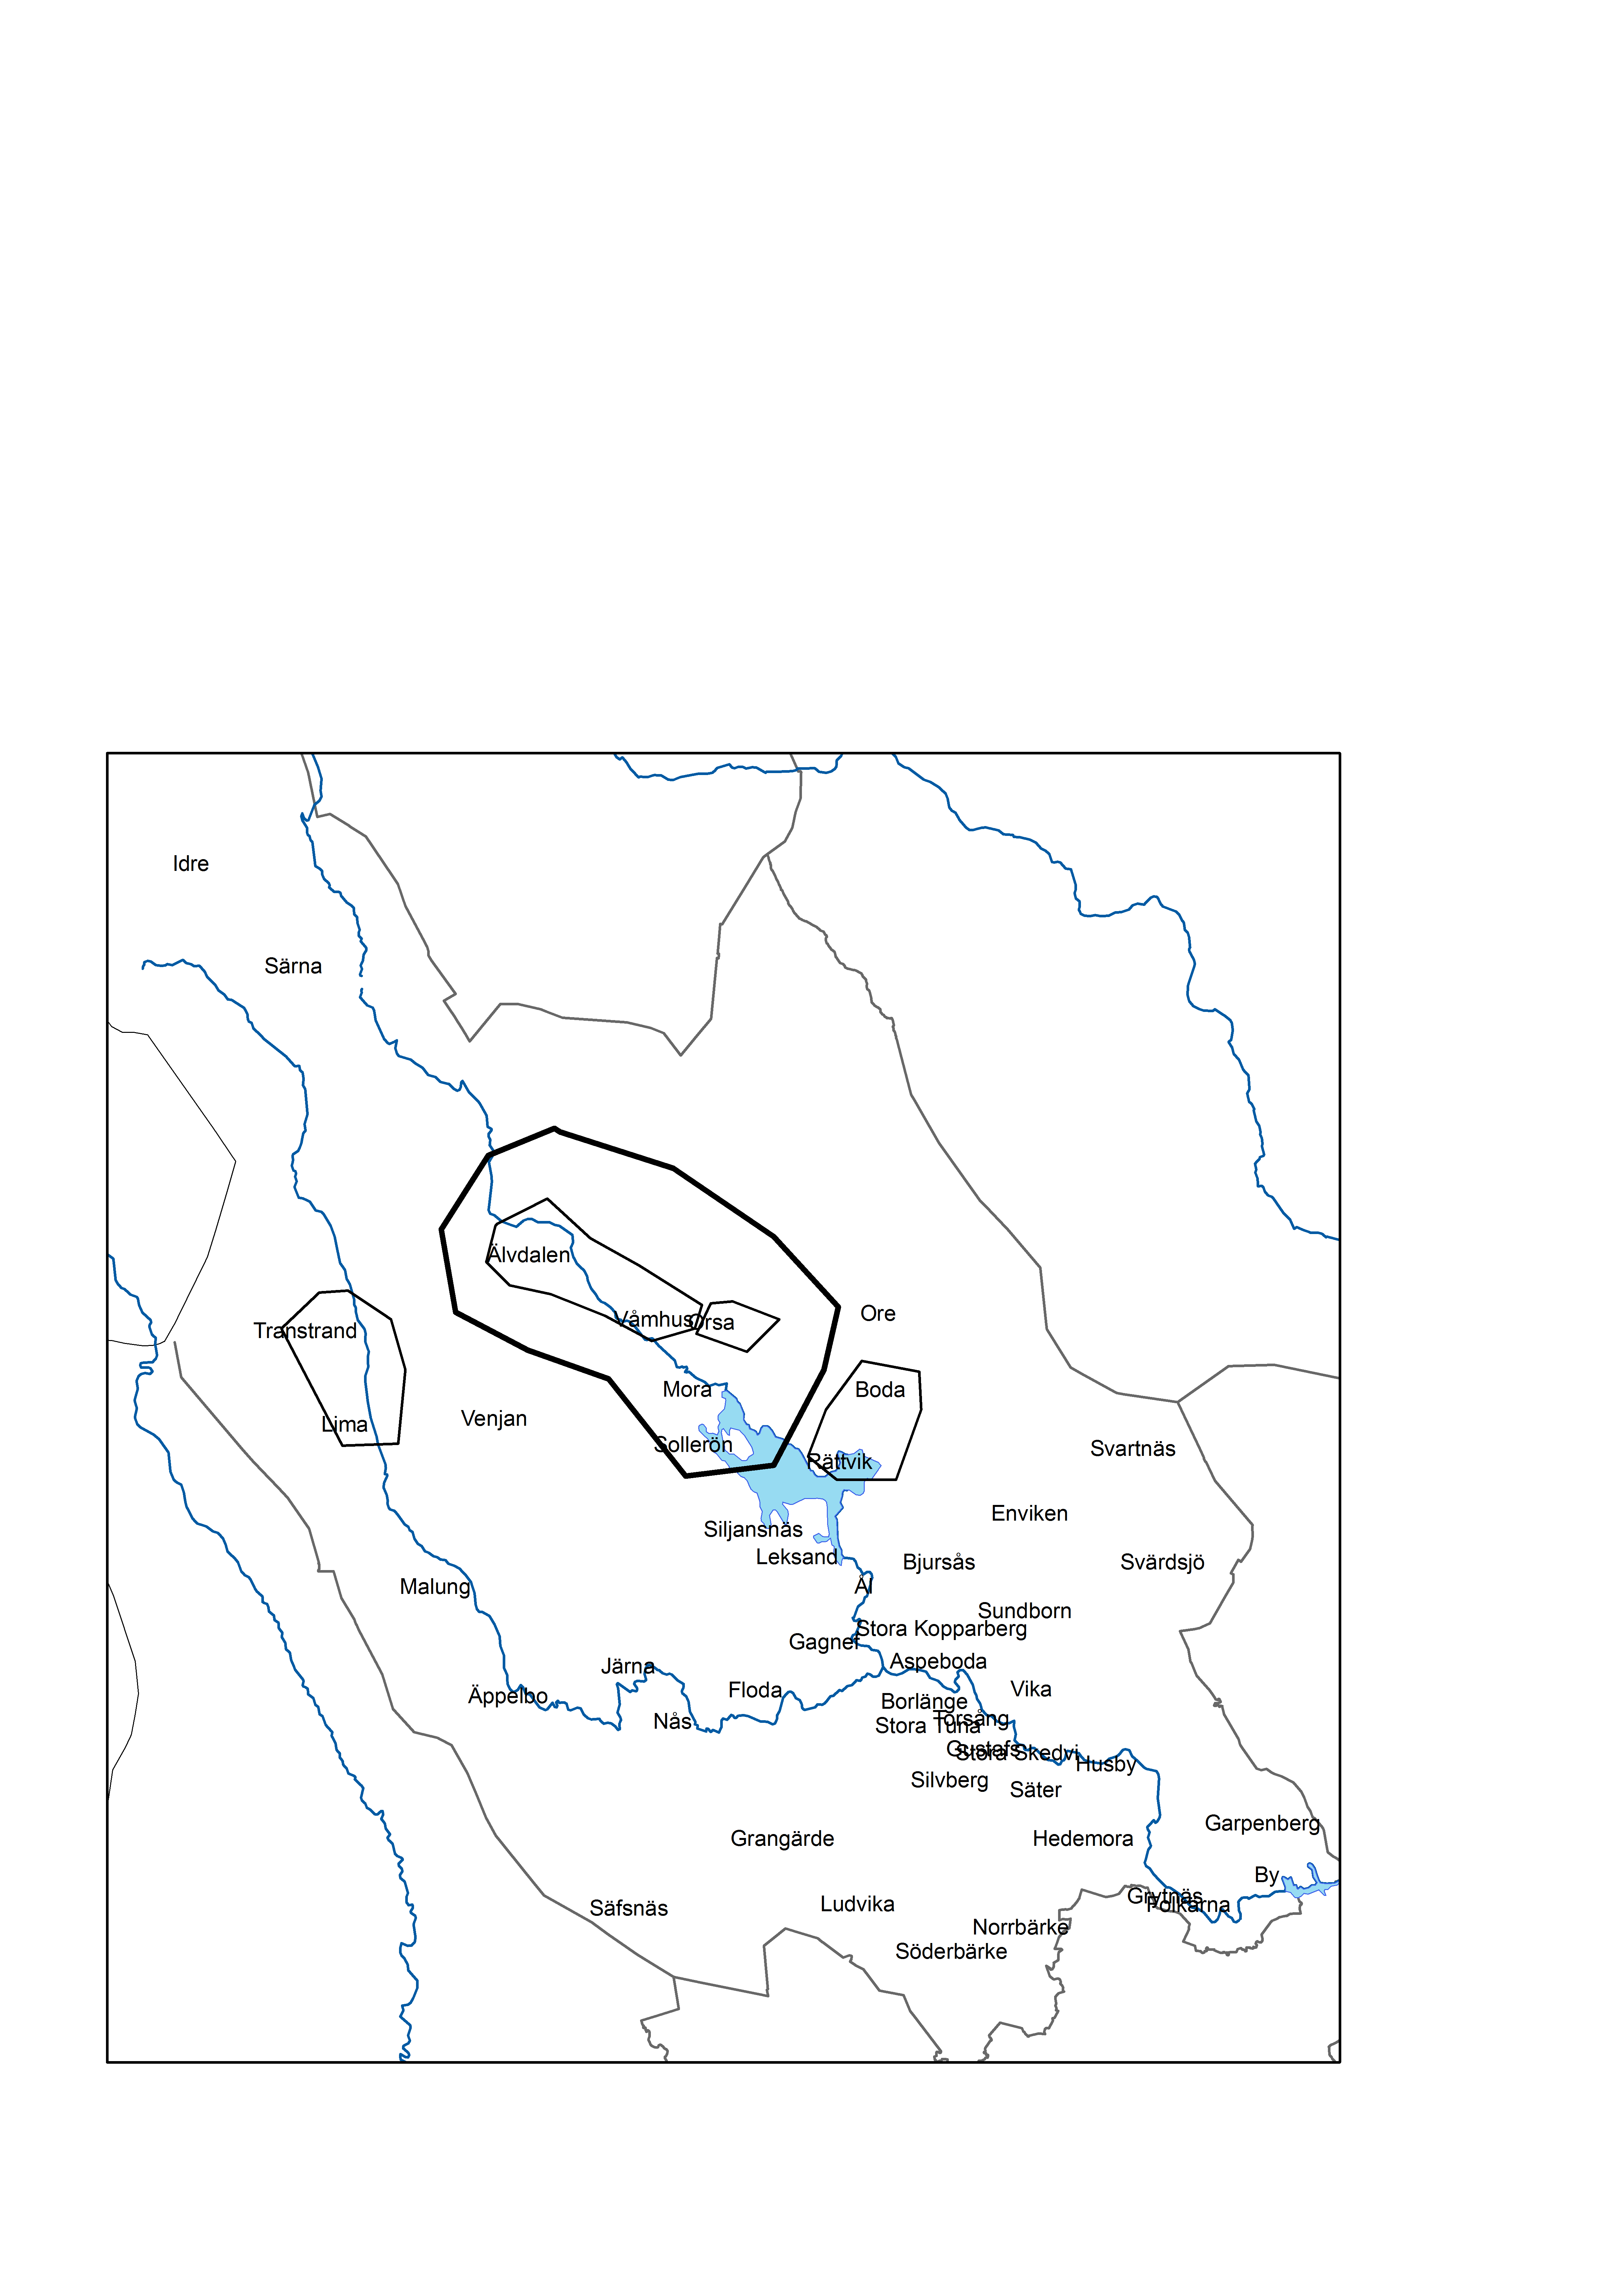
\includegraphics[height=.3\textheight]{figures/8_DalarnaRealistic}
\caption{A more realistic view of Dalecarlian vernaculars.}
\label{map:7}

\end{figure}

\subsection{ Trans-Baltic Swedish}

The Swedish-speaking minority in Finland is comprised of about 260,000 persons. While Standard Finland Swedish differs from “Sweden Swedish” mainly in pronunciation and to some extent in vocabulary, the spoken vernaculars often differ very much from the national standards. 

Until the Second World War, Swedish was also spoken along the coast of Estonia by some 7,000 people, but most of them emigrated to Sweden during the war. During Soviet times, it was generally thought that there were no Swedish speakers left in Estonia but it is now known that a couple of hundred are still there.

In the 18\textsuperscript{th} century, the Russian Empress Catherine the Great moved a number of Swedish-speaking peasants from Estonia to Ukraine, where they lived in a village called “Gammalsvenskby” in Swedish. The majority of the inhabitants of this village emigrated in the 1920s (mainly to Sweden and Canada), but again, there is still a handful of Swedish speakers there. (One of the texts in the Cat Corpus is in the Gammalsvenskby vernacular, which is confusingly called \textstyleLinguisticExample{gammalsvenska} ‘Old Swedish’.)

The Swedish settlements on the east side of the Baltic derive from the Middle Ages, probably starting in the 12\textsuperscript{th} century, while the Åland islands had a Scandinavian population much earlier. It may actually be misleading to think of the four geographically separate areas of Österbotten, southern Finland, coastal Estonia, and Åland as a dialectological unit, since contacts across the Baltic have been at least as important as contacts between the areas. From the point of view of the phenomena treated in this book, Ostrobothnian behaves much more like the Northern Swedish vernaculars than the other Trans-Baltic regions.

